	\subsection{UC 4 - Impostazioni account}

		\begin{figure}[H]
			\centering
			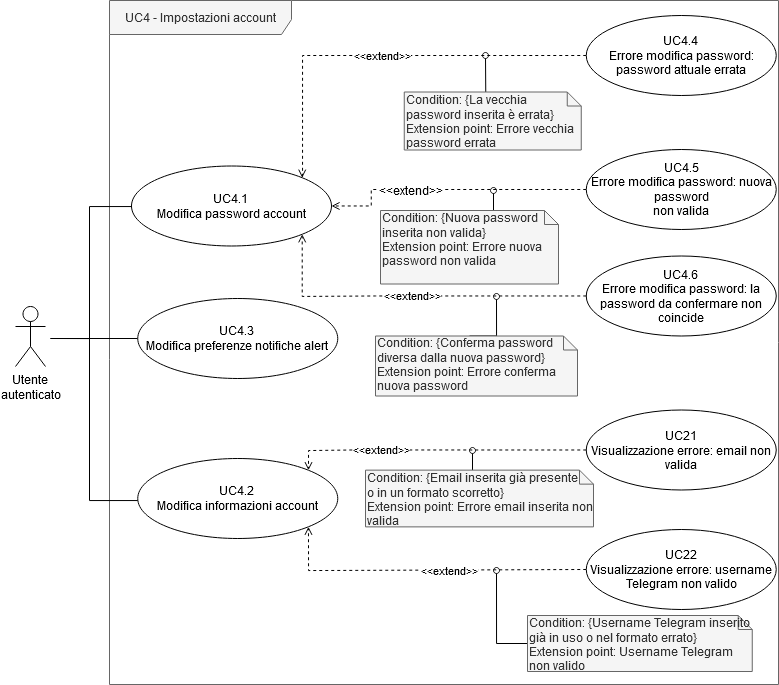
\includegraphics[scale=0.60]{res/images/uc4}
			\caption{Diagramma che riassume le interazioni con le impostazioni del proprio account.}
		\end{figure}

		\begin{itemize}
			\item \textbf{attori primari:} utente autenticato;
			\item \textbf{descrizione:} l'utente ha la possibilità di gestire le proprie impostazioni account, tra cui la modifica della password, le preferenze di notifica e le informazioni a lui associate;
			\item \textbf{precondizione:} l'utente risulta autenticato all'interno della web app;
			\item \textbf{postcondizione:} l'utente ha aggiornato le proprie impostazioni;
			\item \textbf{scenario principale:}
			\begin{enumerate}
				\item{l'utente naviga all'interno delle impostazioni del proprio account;}
				\item{l'utente modifica le proprie impostazioni;}
				\item{l'utente ha aggiornato le proprie impostazioni.}
			\end{enumerate}
		\end{itemize}


			\subsubsection{UC 4.1 - Modifica password account}
			\begin{itemize}
				\item \textbf{attori primari:} utente autenticato;
				\item \textbf{descrizione:} l'utente può cambiare la password associata al proprio account;
				\item \textbf{precondizione:} l'utente naviga all'interno delle sue impostazioni;
				\item \textbf{postcondizione:} l'utente ha cambiato la propria password;
				\item \textbf{scenario principale:}
				\begin{enumerate}
					\item l'utente deve inserire dei campi obbligatori per proseguire;
					\item l'utente inserisce il campo per la password attuale (UC 4.1.1);
					\item l'utente inserisce il campo per la nuova password (UC 4.1.2);
					\item l'utente inserisce il campo per la conferma della nuova password (UC 4.1.3);
					\item l'utente ha cambiato la propria password;
				\end{enumerate}
				\item \textbf{estensioni:}
					\begin{itemize}
						\item errore modifica password: password attuale errata (UC 4.4);
						\item errore modifica password: nuova password non valida (UC 4.5);
						\item errore modifica password: la password da confermare non coincide con la nuova password (UC 4.6).
					\end{itemize}
			\end{itemize}

				\paragraph{UC 4.1.1 - Inserimento password attuale}
				\begin{itemize}
					\item \textbf{attori primari:} utente autenticato;
					\item \textbf{descrizione:} per proseguire nella modifica password, l'utente deve inserire la sua password attuale associata all'account. Il campo è obbligatorio;
					\item \textbf{precondizione:} l'utente è all'interno delle sue impostazioni account;
					\item \textbf{postcondizione:} l'utente ha compilato il campo richiesto;
					\item \textbf{scenario principale:}
					\begin{enumerate}
						\item l'utente compila il campo per la password attuale.
					\end{enumerate}
				\end{itemize}

				\paragraph{UC 4.1.2 - Inserimento nuova password}
				\begin{itemize}
					\item \textbf{attori primari:} utente autenticato;
					\item \textbf{descrizione:} per proseguire nella modifica password, l'utente deve scegliere e inserire una nuova password. Il campo è obbligatorio;
					\item \textbf{precondizione:} l'utente è all'interno delle sue impostazioni account;
					\item \textbf{postcondizione:} l'utente ha compilato il campo richiesto;
					\item \textbf{scenario principale:}
					\begin{enumerate}
						\item l'utente compila il campo per la nuova password.
					\end{enumerate}
				\end{itemize}

				\paragraph{UC 4.1.3 - Inserimento conferma nuova password}
				\begin{itemize}
					\item \textbf{attori primari:} utente autenticato;
					\item \textbf{descrizione:} per proseguire nella modifica password, l'utente deve ripetere la nuova password scelta. Il campo è obbligatorio;
					\item \textbf{precondizione:} l'utente è all'interno delle sue impostazioni account;
					\item \textbf{postcondizione:} l'utente ha compilato il campo richiesto;
					\item \textbf{scenario principale:}
					\begin{enumerate}
						\item l'utente compila il campo per la conferma della nuova password.
					\end{enumerate}
				\end{itemize}

			\subsubsection{UC 4.2 - Modifica informazioni account}
			\begin{itemize}
				\item \textbf{attori primari:} utente autenticato;
				\item \textbf{descrizione:} l'utente può modificare le proprie informazioni associate all'account;
				\item \textbf{precondizione:} l'utente naviga all'interno delle sue impostazioni;
				\item \textbf{postcondizione:} l'utente ha cambiato le proprie informazioni account;
				\item \textbf{scenario principale:}
				\begin{enumerate}
					\item l'utente deve inserire dei campi per proseguire;
					\item l'utente modifica il campo relativo alla propria email (UC 4.2.1);
					\item l'utente modifica il campo relativo allo username di \glock{Telegram} (UC 4.2.2);
					\item l'utente seleziona la preferenza per l'abilitazione dell'autenticazione a due fattori (UC 4.2.3);
					\item l'utente ha cambiato le proprie informazioni associate al suo account;
				\end{enumerate}
				\item \textbf{estensioni:}
					\begin{itemize}
						\item L'utente inserisce un'email non valida (UC 21);
						\item L'utente inserisce uno username \glock{Telegram} non valido (UC 22).
					\end{itemize}
			\end{itemize}

				\paragraph{UC 4.2.1 - Modifica della propria email}
				\begin{itemize}
					\item \textbf{attori primari:} utente autenticato;
					\item \textbf{descrizione:} per proseguire nella modifica delle informazioni, l'utente deve modificare il campo della propria email. Il campo è obbligatorio;
					\item \textbf{precondizione:} l'utente è all'interno delle sue impostazioni account;
					\item \textbf{postcondizione:} l'utente ha compilato il campo richiesto;
					\item \textbf{scenario principale:}
					\begin{enumerate}
						\item l'utente compila il campo per la email.
					\end{enumerate}
				\end{itemize}

				\paragraph{UC 4.2.2 - Modifica dello username Telegram}
				\begin{itemize}
					\item \textbf{attori primari:} utente autenticato;
					\item \textbf{descrizione:} per proseguire nella modifica delle informazioni, l'utente deve modificare il proprio username \glock{Telegram}. Il campo è obbligatorio;
					\item \textbf{precondizione:} l'utente è all'interno delle sue impostazioni account;
					\item \textbf{postcondizione:} l'utente ha compilato il campo richiesto;
					\item \textbf{scenario principale:}
					\begin{enumerate}
						\item l'utente compila il campo dello username \glock{Telegram}.
					\end{enumerate}
				\end{itemize}

				\paragraph{UC 4.2.3 - Modifica delle preferenze per l'autenticazione a due fattori}
				\begin{itemize}
					\item \textbf{attori primari:} utente autenticato;
					\item \textbf{descrizione:} per proseguire nella modifica delle informazioni, l'utente deve selezionare le preferenze per l'abilitazione o meno dell'autenticazione a due fattori con \glock{Telegram}. Le preferenze disponibili sono:
					\begin{itemize}
						\item abilitata;
						\item disabilitata;
					\end{itemize}
					\item \textbf{precondizione:} l'utente è all'interno delle sue impostazioni account;
					\item \textbf{postcondizione:} l'utente ha compilato il campo richiesto;
					\item \textbf{scenario principale:}
					\begin{enumerate}
						\item l'utente seleziona la preferenza per l'autenticazione a due fattori.
					\end{enumerate}
				\end{itemize}


			\subsubsection{UC 4.3 - Modifica preferenze notifiche alert}
			\begin{itemize}
				\item \textbf{attori primari:} utente autenticato;
				\item \textbf{descrizione:} l'utente può modificare le preferenze dei singoli alert che gli sono stati attivati;
				\item \textbf{precondizione:} l'utente naviga all'interno delle sue impostazioni;
				\item \textbf{postcondizione:} l'utente ha cambiato le proprie preferenze per gli alert;
				\item \textbf{scenario principale:}
				\begin{enumerate}
					\item{l'utente seleziona la preferenza di uno o più alert, in base a quelli disponibili;}
					\item{le preferenze alert dell'utente vengono aggiornate.}
				\end{enumerate}
			\end{itemize}

			\subsubsection{UC 4.4 Errore modifica password: password attuale errata}
			\begin{itemize}
				\item \textbf{attori primari:} utente autenticato;
				\item \textbf{descrizione:} durante la modifica della password, il sistema rileva che la password attualmente associata all'account non è valida;
				\item \textbf{precondizione:} l'utente ha compilato i campi richiesti e il sistema elabora la richiesta;
				\item \textbf{postcondizione:} viene visualizzato un messaggio di errore specifico;
				\item \textbf{scenario principale:}
				\begin{enumerate}
					\item il sistema sta elaborando la richiesta;
					\item viene visualizzato un messaggio di errore che segnala che la password attuale è errata.
				\end{enumerate}
			\end{itemize}

			\subsubsection{UC 4.5 Errore modifica password: nuova password non valida}
			\begin{itemize}
				\item \textbf{attori primari:} utente autenticato;
				\item \textbf{descrizione:} durante la modifica della password, il sistema rileva che la nuova password scelta non è valida, dal momento che potrebbe essere uguale a quella attuale o troppo corta;
				\item \textbf{precondizione:} l'utente ha compilato i campi richiesti e il sistema elabora la richiesta;
				\item \textbf{postcondizione:} viene visualizzato un messaggio di errore specifico;
				\item \textbf{scenario principale:}
				\begin{enumerate}
					\item il sistema sta elaborando la richiesta;
					\item viene visualizzato un messaggio di errore che segnala che la nuova password non è valida per uno dei seguenti motivi:
					\begin{itemize}
						\item è troppo corta (è composta da meno di 6 caratteri);
						\item è uguale alla password attuale.
					\end{itemize}
				\end{enumerate}
			\end{itemize}

			\subsubsection{UC 4.6 - Errore modifica password: la password da confermare non coincide}
			\begin{itemize}
				\item \textbf{attori primari:} utente autenticato;
				\item \textbf{descrizione:} durante la modifica della password, il sistema rileva che la nuova password scelta non coincide con la password riportata in conferma password;
				\item \textbf{precondizione:} l'utente ha compilato i campi richiesti e il sistema elabora la richiesta;
				\item \textbf{postcondizione:} viene visualizzato un messaggio di errore specifico;
				\item \textbf{scenario principale:}
				\begin{enumerate}
					\item il sistema sta elaborando la richiesta;
					\item viene visualizzato un messaggio di errore che segnala che la password attuale è errata.
				\end{enumerate}
			\end{itemize}
